\documentclass{article}

\oddsidemargin0mm
\evensidemargin0mm
\topmargin-20mm
\textwidth160mm
\textheight240mm
\parindent0pt

\newcommand{\C}{\mathbb{C}}
\newcommand{\N}{\mathbb{N}}
\newcommand{\Z}{\mathbb{Z}}
\newcommand{\Q}{\mathbb{Q}}
\newcommand{\R}{\mathbb{R}}
\newcommand{\K}{\mathbb{K}}
\usepackage[ngerman]{babel}   % provide non-american language - new german
\usepackage[ansinew]{inputenc} % nur fuer schoene Umlaute ;)
\usepackage{lscape}
\usepackage{multirow}
\usepackage{expdlist}
%\usepackage{bigstrut} % \bigstrut in Tabellenzeilen, deren hochgestellte Eintraege von der \hline drueber durchgestrichen werden
\usepackage{amsmath, amsthm, amssymb}
\usepackage{stmaryrd}
\usepackage{fancyhdr}
\usepackage{graphicx}
\newcommand{\serie}{3}

\pagestyle{fancy}
\fancyhf{}
\fancyhead[L]{Sebastian D\"orner (180766)} %Kopfzeile links
\fancyhead[C]{Algorithmische Geometrie} %zentrierte Kopfzeile
\fancyhead[R]{Mittwoch} %Kopfzeile rechts
\renewcommand{\headrulewidth}{0.0pt} %obere Trennlinie
\fancyfoot[C]{\thepage} %Seitennummer

\begin{document}
\begin{large}
\textbf{L"osung \"Ubung \serie}\\ \\
\end{large}
\textbf{Aufgabe 1}\\
Sei $q$ der Mittelpunkt zwischen $s_i$ und $s_j$. Wir betrachten den Kreis $C$ um $q$ mit Radius $|\overline{qs_i}|$. Die Strecke $\overline{s_is_j}$ ist Durchmesser von $C$ und somit die l\"angste Strecke im Kreis. Da au\ss erdem $s_j$ der n\"achstgelegene Punkt aus $S\setminus \{s_i\}$ zu $s_i$ ist, kann kein anderer Punkt aus $S$ im Kreis sein. Somit ist $C$ der Leerkreis von $q$ bez\"uglich $S$. Also gibt es einen Punkt $q$, sodass $C_S(q)$ nur $s_i$ und $s_j$ enth\"alt, jedoch keinen anderen Punkt aus $S$. Dies ist aber nach einem Satz aus der Vorlesung genau dann der Fall, wenn $\overline{s_is_j}$ eine Kante im Delauny-Diagramm ist. Dann muss $\overline{s_is_j}$ aber auch zur Delauny-Triangulierung $D(S)$ geh\"oren.\qed\\

\textbf{Aufgabe 2}\\
Angenommen der Mittelpunkt $Q$ des Largest Empty Circle l\"age innerhalb einer Voronoi-Region $R$. Sei $P$ das Zentrum dieser Voronoi-Region. Da $Q$ echt innerhalb $R$ liegt, k\"onnen wir $Q$ entlang der $\overline{PQ}$ unterst\"utzenden gerichteten Gerade verschieben, ohne $R$ zu verlassen. Da sich dabei der Abstand von $P$ vergr\"o\ss ert, aber $P$ noch immer der n\"achste Punkt aus $S$ zu $Q$ ist,  kann $Q$ entgegen der Annahme nicht der Mittelpunkt des Largest Empty Circle sein. Somit war unsere Annahme, der Mittelpunkt des LEC l\"age innerhalb einer Voronoi-Region, falsch. Weil der Mittelpunkt nach Definition aber Teil der konvexen H\"ulle sein muss, liegt $Q$ entweder auf einer Voronoi-Kante oder auf dem Rand der konvexen H\"ulle.\qed\\

\textbf{Aufgabe 3}\\
Die ersten drei Kantenmengen sind keine Delauny-Triangulierungen, die letzte hingegen schon:

\begin{figure}[h]
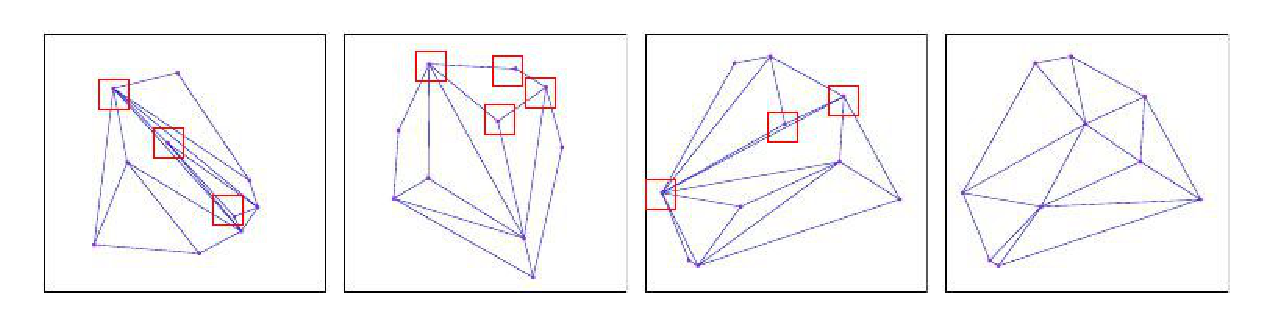
\includegraphics[width=\textwidth]{a3}
\end{figure}
In Kantenmenge 1 und 3 kann enth\"alt der Umkreis der markierten Punkte einen weiteren Punkt. In Kantenmenge zwei bilden die markierten Punkte ein Viereck, das nicht trianguliert ist. Somit handelt es sich gar nicht um eine Triangulation.\\

\textbf{Aufgabe 4}\\
Da die Punkte in allgemeiner Lage sind ist der duale Graph zum Voronoi-Diagramm eine Delauny-Triangulierung. Analog zu Aufgabe 2.6 zeigen wir, dass der durchschnittliche Grad eines Knotens im dualen Graphen kleiner als sechs ist: $\displaystyle \frac{\sum\limits_{v\in V} Grad(v)}{v} = \frac{2e}{v} = \frac{6v -6 -2k}{v} < 6$. Somit muss es einen Knoten geben, dessen Grad echt kleiner als sechs ist. Im urspr\"unglichen Graphen entspricht dieser Knoten aber einer Voronoi-Region, die durch maximal 5 Voronoi-Kanten begrenzt ist.\qed\\

\textbf{Aufgabe 5}\\
\begin{itemize}
\item[(a)] Wir f\"uhren drei Orientierungstests durch, indem wir die folgenden Determinanten berechnen:\\
$\left|\begin{array}{ccc}1 & q_{1x} & q_{1y} \\ 1 & q_{2x} & q_{2y} \\ 1 & p_{x} & p_{y} \end{array}\right|$,
$\left|\begin{array}{ccc}1 & q_{2x} & q_{2y} \\ 1 & q_{3x} & q_{3y} \\ 1 & p_{x} & p_{y} \end{array}\right|$,
$\left|\begin{array}{ccc}1 & q_{3x} & q_{3y} \\ 1 & q_{1x} & q_{1y} \\ 1 & p_{x} & p_{y} \end{array}\right|$ Der Punkt liegt genau dann im Dreieck, wenn alle Determinanten positiv oder alle Determinanten negativ sind. (Es kann nur ein Fall auftreten, je nach Anordnung der Eckpunkte.)
\item[(b)] Wir berechnen die barizentrischen Koordinaten von $P$ durch L\"osung des Gleichungssystems:
\begin{eqnarray*}
p_x &=& \lambda_1q_{1,x} + \lambda_3q_{3,x} + \lambda_3q_{3,x}\\
p_y &=& \lambda_1q_{1,y} + \lambda_3q_{3,y} + \lambda_3q_{3,y}\\
1 &=& \lambda_1 + \lambda_2 + \lambda_3
\end{eqnarray*}
$P$ ist im Dreieck gdw. $0< \lambda_1, \lambda_2, \lambda_3 <1$
\end{itemize}

\end{document}
